%% ==============================================================================
%%
%%  Document settings and macro definitions
%%
%% ==============================================================================

\documentclass[a4paper,10pt,bibtotoc]{scrartcl}
\usepackage{a4wide,usg}
\usepackage{draftcopy}
\usepackage{upgreek}

\newcommand\sumline[2]{%
  \hbox to \linewidth{%
    \strut
    \parbox[t]{.85\linewidth}{\strut #1\strut}\hss
    \parbox[t]{.15\linewidth}{\raggedleft\strut #2\strut}%
  }
}

\newcommand\kw[0]{$KW$}

%% Do NOT remove: required to extract SVN information
\svnInfo $Id$

%% Adjust page footer
\fancyfoot[LE,LO]{LOFAR-USG-ICD-001: TBB Time-Series Data}
\fancyfoot[RE,RO]{\textsc{lofar} Project}

%% ==============================================================================
%%
%%  Document
%%
%% ==============================================================================

\begin{document}

\title{LOFAR Data Format ICD \\ TBB Time-Series Data \\
  {\normalsize Document ID: LOFAR-USG-ICD-001} \\
  {\normalsize Version 3.04.01} \\
  {\normalsize SVN Repository Revision: \svnInfoMaxRevision}}
\author{ \parbox{\linewidth}{\centering L.~B\"ahren,  M.~van~den~Akker, K.~Anderson, A.~Corstanje, A.~Horneffer, J.~Masters, L.~Connor, S.~ter~Veen, G.A.~Renting } }
\date{\small{SVN Date: \svnInfoMaxToday}}

\maketitle

\tableofcontents

\listoffigures

\listoftables

\clearpage

%% ______________________________________________________________________________
%%                                                                  Change record


\section*{Change record}
\addcontentsline{toc}{section}{Change record}


\subsection{Version 1.x}

\subsubsection*{Notes for Version 1.0 $\rightarrow$ Version 1.1}

\begin{enumerate}
\item \textit{Reorganisation of the placement of attributes describing
    basic properties of the observation from which the dataset has
    originated.} \\
  Some part of the information which originally was supposed to be stored within
  the Station groups should be shifted upwards to the root group of the file.
  \begin{itemize}
  \item[\underline{old}:]
    {\small
\begin{verbatim}
/
|-- STATION_001                         ... Group
|   |-- TELESCOPE                       ... Attribute       ... string
|   |-- OBSERVER                        ... Attribute       ... string
|   |-- PROJECT                         ... Attribute       ... string
|   |-- OBSERVATION_ID                  ... Attribute       ... string
|   |-- OBSERVATION_MODE                ... Attribute       ... string
|   `
|-- STATION_002                         ... Group
|   |-- TELESCOPE                       ... Attribute       ... string
|   |-- OBSERVER                        ... Attribute       ... string
|   |-- PROJECT                         ... Attribute       ... string
|   |-- OBSERVATION_ID                  ... Attribute       ... string
|   |-- OBSERVATION_MODE                ... Attribute       ... string
|   `
\end{verbatim}}
  \item[\underline{new}:]
    {\small
\begin{verbatim}
/
|-- TELESCOPE                           ... Attribute       ... string
|-- OBSERVER                            ... Attribute       ... string
|-- PROJECT                             ... Attribute       ... string
|-- OBSERVATION_ID                      ... Attribute       ... string
|-- OBSERVATION_MODE                    ... Attribute       ... string
|-- STATION_001                         ... Group
|   |
|   `
|-- STATION_002                         ... Group
|   |
|   `
\end{verbatim}}
  \end{itemize}
\item \textit{Proper handling of coordinates} \\
    The motivation for this changes are in the fact, that for proper
    representation of a direction or position information more but just the
    numerical value is required -- thus the additional information should be
    stored within the file as well, as compared to simply assuming the stored
    data adhere to a certain convention (which on the other hand they still
    should).
  \begin{itemize}
  \item[\underline{old}:]
    {\small
\begin{verbatim}
/
|-- STATION_001                         ... Group
|   |-- BEAM_DIRECTION                  ... Attribute       ... array<double,1>
|   |-- 001000000                       ... Dataset
|   |   |-- ANTENNA_POSITION            ... Attribute       ... array<double,1>
|   |   |-- ANTENNA_ORIENTATION         ... Attribute       ... array<double,1>
|   |   |-- SAMPLE_FREQUENCY            ... Attribute       ... double
|
\end{verbatim}}
  \item[\underline{new}:]
    {\small
\begin{verbatim}
/
|-- STATION_001                         ... Group
|   |-- STATION_POSITION_VALUE          ... Attribute       ... array<double,1>
|   |-- STATION_POSITION_UNIT           ... Attribute       ... string
|   |-- STATION_POSITION_FRAME          ... Attribute       ... string
|   |-- BEAM_DIRECTION_VALUE            ... Attribute       ... array<double,1>
|   |-- BEAM_DIRECTION_UNIT             ... Attribute       ... string
|   |-- BEAM_DIRECTION_FRAME            ... Attribute       ... string
|   |-- 001000000                       ... Dataset
|   |   |-- ANTENNA_POSITION_VALUE      ... Attribute       ... array<double,1>
|   |   |-- ANTENNA_POSITION_UNIT       ... Attribute       ... string
|   |   |-- ANTENNA_POSITION_FRAME      ... Attribute       ... string
|   |   |-- ANTENNA_ORIENTATION_VALUE   ... Attribute       ... array<double,1>
|   |   |-- ANTENNA_ORIENTATION_UNIT    ... Attribute       ... string
|   |   |-- ANTENNA_ORIENTATION_FRAME   ... Attribute       ... string
|   |   |-- SAMPLE_FREQUENCY_VALUE      ... Attribute       ... double
|   |   |-- SAMPLE_FREQUENCY_UNIT       ... Attribute       ... string
|
\end{verbatim}}
  \end{itemize}
\item \textit{Sensible (default) values} \\
  One of the -- at least temporary -- problems is, that some of the values to be
  stored within the HDF5 file are not available (yet) at the time of creating the
  file on disk. Therefore at least sensible default values/settings should be used
  to enable correct interpretation of the dataset; e.g. position information at a
  later point will be retrieved from the central parameter database, but until then
  the attributes should be filled already with placeholder values which agree with
  the conventions of the Measures framework. If a value in fact is undefined, it
  should be clearly marked as such by using \verb|UNDEFINED| (in case of a string
  valued attribute).
  {\small
\begin{verbatim}
/
|-- STATION_001
|   |-- STATION_POSITION_VALUE         ... array<double,1>    ...  {x,y,z}
|   |-- STATION_POSITION_UNIT          ... string             ...  "m"
|   |-- STATION_POSITION_FRAME         ... string             ...  "ITRF"
|   |-- BEAM_DIRECTION_VALUE           ... array<double,1>    ...  {0,90}
|   |-- BEAM_DIRECTION_UNIT            ... string             ...  "deg"
|   |-- BEAM_DIRECTION_STRING          ... string             ...  "UNDEFINED"
|   |-- 001000000
|   |   |-- ANTENNA_POSITION_VALUE     ... array<double,1>    ...  {x,y,z}
|   |   |-- ANTENNA_POSITION_UNIT      ... string             ...  "m"
|   |   |-- ANTENNA_POSITION_FRAME     ... string             ...  "ITRF"
|   |   |-- ANTENNA_ORIENTATION_VALUE  ... array<double,1>    ...  {x,y,z}
|   |   |-- ANTENNA_ORIENTATION_UNIT   ... string             ...  "m"
|   |   |-- ANTENNA_ORIENTATION_FRAME  ... string             ...  "ITRF"
|   |   |-- FEED                       ... string             ...  "UNDEFINED"
|   |   |-- NYQUIST_ZONE               ... uint               ...  1
|   |   |-- SAMPLE_FREQUENCY_UNIT      ... string             ...  "Hz"
|
\end{verbatim}}
\end{enumerate}

\subsubsection*{Version 1.1 $\rightarrow$ Version 1.2}

\begin{enumerate}
\item \textit{Parametrization of coordinates} \\
  While the basic scheme for encoding and later reconstruction of the
  coordinate information remains unaltered, a minor detail was overlooked in
  the previous revision: in the general case one can not assume, that all
  values of a coodinate are given in the same physica unit. While e.g. for
  a simple direction -- as described by two angles -- the units are identical,
  this is not longer the when e.g. describing a position on the surface of
  the Earth (e.g. the position of the telescope). The simplest example for
  the latter case is the WGS84 system: in this a position is described by
  two angles and a height relative to the model geoid -- therefore using
  \verb|[deg,deg,m]| as units -- hence the required modification in the data
  format to take this into account.
  \begin{itemize}
  \item[\underline{old}:]
    {\small
\begin{verbatim}
/
|-- STATION_001                         ... Group
|   |-- STATION_POSITION_UNIT           ... Attribute       ... string
|   |-- BEAM_DIRECTION_UNIT             ... Attribute       ... string
|   |-- 001000000                       ... Dataset
|   |   |-- ANTENNA_POSITION_UNIT       ... Attribute       ... string
|   |   |-- ANTENNA_ORIENTATION_UNIT    ... Attribute       ... string
|
\end{verbatim}}
  \item[\underline{new}:]
    {\small
\begin{verbatim}
/
|-- STATION_001                         ... Group
|   |-- STATION_POSITION_UNIT           ... Attribute       ... array<string,1>
|   |-- BEAM_DIRECTION_UNIT             ... Attribute       ... array<string,1>
|   |-- 001000000                       ... Dataset
|   |   |-- ANTENNA_POSITION_UNIT       ... Attribute       ... array<string,1>
|   |   |-- ANTENNA_ORIENTATION_UNIT    ... Attribute       ... array<string,1>
|
\end{verbatim}}
  \end{itemize}
  As a consequence the values actually stored as attributes can look something
  like:
{\small
\begin{verbatim}
/
|-- STATION_001
|   |-- STATION_POSITION               ... array<double,1>    ...  {10,-6,50}
|   |-- STATION_POSITION_UNIT          ... array<string,1>    ...  {"m","deg","deg"}
|   |-- STATION_POSITION_FRAME         ... string             ...  "WGS84"
|   |
\end{verbatim}}
\end{enumerate}

\subsubsection*{Version 1.2 $\rightarrow$ Version 1.x}

{\small
\begin{verbatim}
BEAM_WIDTH_VALUE
BEAM_WIDTH_UNIT
\end{verbatim}}


\begin{center}
  %% Table head
  \tablefirsthead{
    \hline
    \textsc{Version} & \textsc{Date} & \textsc{Sections} & \textsc{Description of changes} \\
    \hline
  }
  \tablehead{
    \multicolumn{4}{r}{\small\textsl{continued from previous page}} \\
    \hline
    \textsc{Version} & \textsc{Date} & \textsc{Sections} & \textsc{Description of changes} \\
    \hline
  }
  %% Table tail
  \tabletail{
    \hline
    \multicolumn{4}{r}{\small\textsl{continued on next page}} \\
  }
  \tablelasttail{\hline}
  %% Table contents
  \begin{supertabular}{lllp{9.5cm}}
    1.00.00 & yyyy-mm-dd & all & Attribute reorganization, ``sensible default values''.\\
    1.01.00 & yyyy-mm-dd & all & Coordinate parametrization.\\
    1.02.00 & 2008-09-08 & -- & Beam parameters. \\
    1.03.00 & 2008-09-08 & --  & --/-- \\
    1.04.00 & 2009-07-08 & all & Reorganization wrt. common ICD format. \\
    1.05.00 & 2009-09-15 & 3, 4.5 & Updated high-level structure; new
    section on trigger table.\\
    1.06.00 & 2010-01-26 & 1, 4, 6 & Added summary of data volumes; update to
    trigger and calibration information; open questions now as
    table. \\
    1.07.00 & 2010-02-03 & 4.5 & Cleaning up of section on trigger table;
    extended list of table columns and description. Removed mentioning
    of Data Visualization Library (DVL). \\
    1.08.00 & 2010-03-16 & all & Merging various comments on the previous
    version of the ICD. Completely reworked section on station trigger. \\
    1.09.00 & 2010-04-14 & 4.3, 6 & Added attribute to station group. Added
    proposal for how to store calibration information as part of the
    station and dipole group; suggesting to replace simple dipole
    dataset by dipole group to take up both time-series data and
    calibration data. \\
    1.10.00 & 2010-04-20 & 4/4.1 & Refactor Root Group  Sec. 4.1
    $\rightarrow$ sec. 4.1.1, 4.1.2. \\
    1.11.00 & 2010-05-14 & 3, 6.2 & Integration suggested changes to dipole
    data structure into the main document. \\
    1.12.00 & 2010-06-29 & \ref{sec:hierarchical structure}, & Rewrite of section
    describing storage of calibration information. Added references. \\
  \end{supertabular}
\end{center}

\subsubsection*{Version 2.0 $\rightarrow$ Version 2.x}

\begin{center}
  %% Table head
  \tablefirsthead{
    \hline
    \textsc{Version} & \textsc{Date} & \textsc{Sections} & \textsc{Description of changes} \\
    \hline
  }
  \tablehead{
    \multicolumn{4}{r}{\small\textsl{continued from previous page}} \\
    \hline
    \textsc{Version} & \textsc{Date} & \textsc{Sections} & \textsc{Description of changes} \\
    \hline
  }
  %% Table tail
  \tabletail{
    \hline
    \multicolumn{4}{r}{\small\textsl{continued on next page}} \\
  }
  \tablelasttail{\hline}
  %% Table contents
  \begin{supertabular}{lllp{9.5cm}}
    2.00.00  & 2010-07-08 & Cover & Changed `revision` to `version`;  updated
   this version number to 2.00.00 for LOFAR ICDs 1 through 7 to put them on the same
   version numbering scheme.\\
    2.01.00 & 2010-07-14 & \ref{sec:station group}, \ref{sec:trigger group}
    & Added \textsl{Acknowledgements} section. Adjusted version
    numbering scheme to include zero-padding. Added \textsl{clock
      offset} attribute. Adusted type of fit parameters in the
    \textsl{Station Trigger Group}. \\
    2.01.01 & 2010-12-07 & all & Using \LaTeX\ package
    \texttt{hyperref} for references, enabling better navigation
    through the document and access to external resources. \\
    2.01.02 & 2011-01-05 & cover & the document Id is HARD. not svnInfo. \\
    2.01.03 & 2011-02-17 & all & Adding document title to page footer. \\
    2.01.04 & 2011-02-28 & all & Fixed data volume estimates, fixed
    naming conventions for Groups and Datasets to UpperCamelCase. \\
    2.01.05 & 2011-03-10 & all & Maintain list of references
    through Bib\LaTeX\ database. \\
    2.01.06 & 2011-03-01 & 4 & Added root group to hold trigger-specific information. \\
    \hline
    \multicolumn{4}{c}{Version upon which the current data-reader is based$^*$}. \\
    \hline
    2.02.01 & 2011-04-20 & all & Strings and string arrays: useage now consistent.\\
    2.02.02 & 2011-05-12 & all & Shifted all 2.01 and earlier changes to the`detailed change log' in the appendix.\\
    && 3 & Added a `data flow' placeholder, and switched the order of the `overview' and `heirarchical structure' subsections.\\
    && 4 & Adjusted the `coordinates subgroup' section in table 1.\\
    && 4 & Removed the group-type for `DumpMetaData' and replaced with `string'.\\
    && 4 & Added `LORA' as a possible `DUMP\_TYPE' value.\\
    && 4 & Ensured all Fields/Keywords are caps only.\\
    && 4 & Changed dimensionality of \verb|BEAM_SHAPE_DATA| to 3 (was 1). Everything is now `BEAM\_SHAPE'/`BeamShape'/`beam shape'.\\
    && 3 \& 4 & Station Trigger Group moved to the `root' directory.\\
    && all & Removed all but the first  `posix-style hierachy' from the document.\\
    && 3,4 & Moved VHECR-specific component of `station trigger group' to the root-level metadata.\\
    2.02.07 & 2011-06-09 & 0,5, A & Re-organised appendices and included full change-log.\\
    2.02.08 & 2011-07-06 & all & Matching up group type attributes and
    notation; consolidation of labels to refer to standard sections
    and tables. \\
    2.02.09 & 2011-09-15 & all & Rework after review.\\ % Needs better description.
    2.02.10 & 2011-12-21 & 0 & Added data type section.\\
            &            & 4 & Added metadata introduction.\\
    2.02.11 & 2012-01-03 & 4 & Added `Manual' as keyword for trigger
    type.\\
    2.02.12 & 2012-01-03 & 4 & Update of optional keywords which are
    now in italic.\\
    2.02.13 & 2012-01-11 & cover & Modification of SVN version information.\\
            &            & 4     & Change \verb|CABLE_DELAY| keyword
                                   to \verb|CABLE_DELAY_VALUE|.\\
    2.02.14 & 2012-01-11 & 4     & Added keyword \verb|DIPOLE_CALIBRATION_DELAY|.\\
    2.02.15 & 2012-01-31 & 4     & Removed of calibration information.\\
            &            &       & Added several keywords to the trigger group and dipole dataset.\\
            &            &       & Updated mandatory/optional
                                   keywords.\\
    2.02.16 & 2012-02-16 & & Renamed \verb|ATTRIBUTE_VALUE| into \verb|ATTRIBUTE|.\\
            &            & & Renamed station group names: \verb|STATION_NNN| $\to$ \verb|AAKKK|\\
    2.02.17 & 2012-02-21 & all & Fixed all quotes for correct forward/backwards orientation.\\
    2.02.18 & 2012-02-24 & all & Added list of figures and list of tables
                                 + update of figure/table captions.\\
    2.02.19 & 2012-03-05 & 5     & Removed section 5 (Interfaces).\\
    2.02.20 & 2012-03-06 & cover & Added draftcopy package for background 'draft' text.\\
    2.02.21 & 2012-03-07 & all   & Removed references to removed section 5 (Interfaces).\\
    2.02.22 & 2012-03-09 & 4     & Added column with software version number to keyword tables.\\
    2.02.23 & 2012-03-20 & 4     & Minor fix in Table~\ref{tab:trigger_types}.\\
    2.02.24 & 2012-06-15 & all   & More consistent naming group names.\\
    2.02.25 & 2012-07-12 & all   & Added minor modifications mentioned in ICD-meeting.\\
    2.02.26 & 2012-07-19 & 4     & Added definition of \verb|SAMPLE_NUMBER| in text.\\
    2.02.27 & 2012-11-13 & 4     & Update of data structure description as they are now in the released DAL / TBB Writer.\\
 \end{supertabular}
\end{center}

$^*$NOTE: P.\ Schellart used this document to design a data-reading program as
of March/April 2011. %
Hence, everything from May onwards is designated as `v2.02'.

\subsubsection*{Version 3.0 $\rightarrow$ Version 3.x}

\begin{center}
  %% Table head
  \tablefirsthead{
    \hline
    \textsc{Version} & \textsc{Date} & \textsc{Sections} & \textsc{Description of changes} \\
    \hline
  }
  \tablehead{
    \multicolumn{4}{r}{\small\textsl{continued from previous page}} \\
    \hline
    \textsc{Version} & \textsc{Date} & \textsc{Sections} & \textsc{Description of changes} \\
    \hline
  }
  %% Table tail
  \tabletail{
    \hline
    \multicolumn{4}{r}{\small\textsl{continued on next page}} \\
  }
  \tablelasttail{\hline}
  %% Table contents
  \begin{supertabular}{lllp{9.5cm}}
    3.00.00 & 2017-11-07 & all   & Changed the document to a subband mode ICD. 
       More cleanup is needed, but the relevant keywords are added. \\
    3.01.00 & 2018-10-24 & all   & Cleanup of the document. \\
    3.02.00 & 2018-10-24 & all   & Changed the document to support both raw voltage time series and subband mode time series. \\
    3.03.00 & 2018-11-08 & 3,4  & Clarified the overview text and re-organised the fields between Dipole Group and Subband dataset. \\
    3.04.00 & 2018-11-16 & 3,4  & Various small changes.\\
    3.04.01 & 2018-11-22 & 4  & Put DAL version 3.3 into the document and made some small typo fixes. Added glossary. \\
 \end{supertabular}
\end{center}


\subsubsection*{Version 4.0 $\rightarrow$ Version 4.x}

\begin{center}
  %% Table head
  \tablefirsthead{
    \hline
    \textsc{Version} & \textsc{Date} & \textsc{Sections} & \textsc{Description of changes} \\
    \hline
  }
  \tablehead{
    \multicolumn{4}{r}{\small\textsl{continued from previous page}} \\
    \hline
    \textsc{Version} & \textsc{Date} & \textsc{Sections} & \textsc{Description of changes} \\
    \hline
  }
  %% Table tail
  \tabletail{
    \hline
    \multicolumn{4}{r}{\small\textsl{continued on next page}} \\
  }
  \tablelasttail{\hline}
  %% Table contents
  \begin{supertabular}{lllp{9.5cm}}
    4.00.00 & 2025-06-13 & all   & Changes for LOFAR2.0. Removed Subband Groups. Introduced \texttt{FieldGroup}. Added keyword \texttt{TILE\_DIPOLES\_ENABLED}. Moved \texttt{DIPOLE\_CALIBRATION} values to a separate group where calibration table can be stored. \\
    4.01.00 & 2018-10-24 & all   & Cleanup of the document. \\
 \end{supertabular}
\end{center}

\input version_numbering

\input types

\input notation


\clearpage

%%_______________________________________________________________________________
%%                                                                   Introduction

\section{Introduction}
\label{sec:introduction}

\subsection{Purpose and scope}
\label{sec:purpose and scope}

This interface control document (ICD) describes the internal structure
of and the interface to the LOFAR time series data as generated by the Transient Buffer Boards (TBB) 
 Time series data -- i.e. the digitised voltage output, as received by the individual
LOFAR dipoles -- represent the primary input data to the CR (Cosmic
Ray) analysis pipeline(s) and have to be considered as the most basic
form in which the received radio signals are present within the LOFAR
system. With the LOFAR 2.0 upgrade, this functionality is known as Transient Buffer (TBuf) 
as they do not have their own separate board.

\subsection{Context and motivation}
\label{sec:context and motivation}

The fundamental difference between analysis for LOFAR Cosmic Ray (CR)
data with respect to other LOFAR Key Science Projects (KSP) is the
fact that processing starts from the raw digitised time-series data
delivered by the individual dipoles of the LOFAR telescope. This
approach is required to provide the necessary time-resolution --
essentially down to the time-interval at which the analog signal is
sampled -- to detect, identify and investigate the radio pulses from
Extensive Air-Showers (EAS) originating form high-energy cosmic rays.

More recently the raw digitised time-series data has also become useful 
in studying the science of lighting and thunderstorms, Fast Radio Bursts (FRB),
and the interaction of neutrinos with the Moon.

Based on a number of considerations we have chosen the HDF5 data
format as common wrapper for the standard LOFAR data products (or at
least a considerable fraction thereof). The goal is to create along
with the definitions of the standard data product also an
infrastructure which will enable LOFAR users to access and manipulate
such data -- this document therefore also serves as reference for the
implementation with the Data Access Library (DAL).

\input applicable_documents

%% ______________________________________________________________________________
%%                                                              Section: Overview

\section{Overview}
\label{sec:overview}

This document is structured as follows: %
Section \ref{sec:structure} will describe fundamental overall
structure, including a statement of the primary data product format,
HDF5. These conventions will also include names, meaning, and physical
units that may be used to generate and interpret the data files. %
Section \ref{sec:detailed structure} will present a detailed
specification for the data, including a description of the structure
of a LOFAR TBB data naming conventions, units, physical quantities. %

\begin{comment}
This is not a finished document. It needs further clarification in the text of what certain values mean, especially in the Trigger Group section.
See the various comment blocks in the text. The definition of the file format itself should be complete however, just not all values equally well documented.
\end{comment}

%%_______________________________________________________________________________
%%                                                       Organisation of the data

\clearpage

\section{Organisation of the data}
\label{sec:structure}

\subsection{High level LOFAR TBB Times-series file structure}

A LOFAR TBB Times-series data file will adhere to the following guidelines:\\

A LOFAR TBB Times-series data file will be defined within the context
of the HDF5 file format.  A LOFAR TBB Time-series HDF5 file structure
will comprise a primary group, a "root group" in HDF5 nomenclature,
which may be considered equivalent to a primary header/data unit (HDU)
of a standard multi-extension FITS file.  This primary group will
consist only of header keywords (“attributes” in HDF5 nomenclature)
describing general properties of an observation, along with pointers
to contained subgroups.  Those subgroups will comprise an arbitrary
number of ``StationGroups'' (see sec~\ref{sec:station group}), where a
Station Group will contain data and meta-data produced by an
individual LOFAR station. Under each Station Group there are one or two more levels
depending on the data taking mode used.

Figure~\ref{fig:TBB_highlevel} shows the basic organisation of the dataset within
the HDF5 format. The hierarchical structure essentially follows the
hierarchical structure of LOFAR itself, i.e. in a top-down approach
from array through stations down to individual dipoles. The grouping
of multiple antennas/dipoles into a station is mirrored by the
collection of dipole datasets into a station group.

\subsection{Overview of TBB Groups}

From version 3 of this document, it is possible to store two variants of TBB data:
\begin{enumerate}
\item \textbf{Raw Voltage Mode} This is the same mode also supported by version 2 of this document. It records the raw voltage per dipole after analog-digital conversion. In older LOFAR documents and software this is often called \emph{transient mode}. With a station clock of 200MHz this has a 5 ns resolution.%
\item \textbf{Subband Mode} This variant is added in version 3 and allows to record each subband separately as complex voltages after the RSP has performed a polyphase filter (PPF) transpose into 512 subbands. The data for the subbands can be frozen with different time delays according to a specified dispersion measure (DM). In some older LOFAR documents and software this is called \emph{spectral mode}. With a station clock of 200 Mhz this has a 5.12 $\upmu$s resolution and up to 512 subbands.%
\end{enumerate}

The structure of the file is subdivided into the following four or five HDF5 group levels, depending on which mode is being used:

\begin{enumerate}
\item \textbf{File Root Group} (\verb|ROOT|). The root level of the file contains the
  majority of associated meta-data, describing the circumstances of
  the observation. These data attributes include observation time
  (start and end), frequency window (high band vs. low band, filters)
  and other important characteristics of the dataset. See
  section \ref{sec:root group} for further details.
\item \textbf{Trigger Group} (\verb|TRIGGER|). This
  group collects parameters generated by the (station-level) trigger
  algorithm. See section \ref{sec:trigger group} for further
  details.
\item \textbf{Station Group} (\verb|STATION_{AAKKK}|). This group serves as a
  common container for the separate sub-tables, which take up data from the
  station calibration and the trigger algorithm. 
  The part between \verb|{...}| represents the station name and consists of 2
  characters (upper case) and three digits (e.g. 'CS001' or 'RS106'). 
  See section \ref{sec:station group} for further details.
\item \textbf{Dipole Dataset/Group} (\verb|DIPOLE_{NNNMMMLLL}|). This group
  collects data on a per-dipole basis starting from the identifiers required for
  the unambiguous identification of an individual dipole within the full LOFAR
  network to the actual sampled wave-form of the EM-field at the position of
  each antenna feed. This group either contains a dataset of the sampled raw voltages after analog-digital conversion
  or serves as a container for separate subtables for each subband in Subband Mode. 
  The part between \verb|{...}| represents the name of the dataset and is
  constructed from the \small \textit{\texttt{STATION\_ID}} (NNN), \verb|RSP_ID|
  (MMM) and \verb|RCU_ID| (LLL). 
  See section \ref{sec:dipole dataset} and \ref{sec:dipole group} for further details.
\item \textbf{Subband Group} (\verb|SB_{BBB}|). In Subband Mode this group contains the complex voltages for each subband. 
  The part between \verb|{...}| represents the the subband on the RCU and contains three digits (e.g. '100' or '106'). 
  See section \ref{sec:subband dataset} for further details.
\end{enumerate}


\begin{comment}
DIPOLE also doesn't seem to be the most accurate name, as we seem to be modelling HBA tiles or LBA dipoles?
\end{comment}

%%_______________________________________________________________________________
%%                                                    Detailed Data Specification


\subsection{Hierarchical structure}
\label{sec:hierarchical structure}

\begin{figure}[htb]
  \centering
  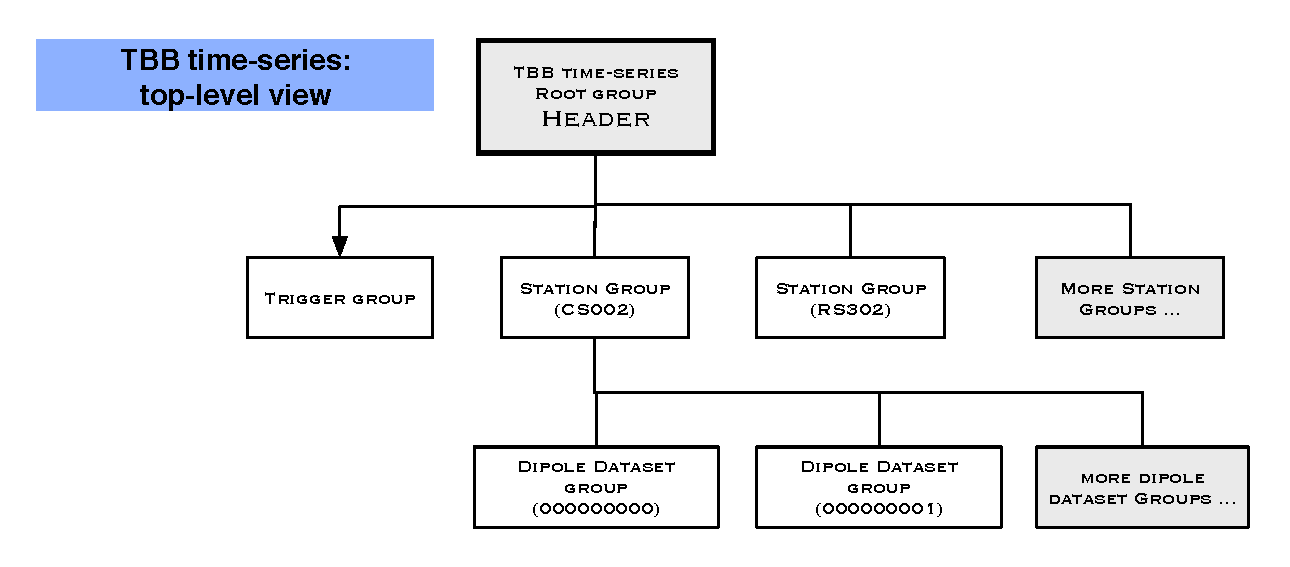
\includegraphics[width=\textwidth]{figures/TBB_highlevel_new.eps}
  \caption[Hierarchical structure of a TBB times-series dataset.]{
    Hierarchical structure of a TBB times-series dataset; the
    internal organization of the data follows the hierarchical
    organization of the LOFAR system.}
  \label{fig:TBB_highlevel}
\end{figure}

{\small
\begin{verbatim}
/                                          ...  Root Group
|-- TRIGGER                                ...  Group
|-- STATION_{AAKKK}                        ...  Group
|   |-- FIELD_XBA                          ...  Group (LBA or HBA)
|   |   |-- DIPOLE_{NNNMMMLLL}                 ...  Dataset     [1D, short] (Raw Voltage Mode)
\end{verbatim}
}

This structure can be represented through HDF5 as a \textsc{posix}-style hierarchy:

Raw Voltage Mode:
\begin{verbatim}
/
/TRIGGER
/STATION_CS002
/STATION_CS002/FIELD_LBA/DIPOLE_000000000
/STATION_CS002/FIELD_LBA/DIPOLE_000000001
/STATION_CS002/FIELD_LBA/DIPOLE_000...
/STATION_CS002/FIELD_HBA/DIPOLE_000000000
/STATION_CS002/FIELD_HBA/DIPOLE_000000001
/STATION_CS002/FIELD_HBA/DIPOLE_000...
/STATION_RS302
/STATION_RS302/FIELD_LBA/DIPOLE_001000000
/STATION_RS302/FIELD_LBA/DIPOLE_...
/STATION_RS302/FIELD_HBA/DIPOLE_001000000
/STATION_RS302/FIELD_HBA/DIPOLE_001...
...
\end{verbatim}


%%______________________________________________________________________________
%%                                                   Detailed Data Specification

\clearpage

\section{Detailed Data Specification}
\label{sec:detailed structure}

\input metadata_intro

\subsection{The Root Group}
\label{sec:root group}

The LOFAR file hierarchy begins with the top level \verb|`Root Group'|.  This is
the file entry point for the data, and the file node by which navigation of
the data is provided. The \texttt{Root Group} will comprise a set of attributes
that describe the underlying file structure, observational metadata, the LOFAR
TBB data, as well as providing hooks to all groups attached to the \texttt{Root
  Group}.

This section will specify two sets of attributes that will appear in
the \texttt{Root Group}: a set of \cla\ (CLA) that will be common to
all LOFAR science data products, and a set of attributes that are
specific to LOFAR TBB Time-series data.  Though these attributes will
all appear together in the \texttt{Root} attribute set, they are
separated in this document in order to demarcate those general LOFAR
attributes that are applicable across all data, and those attributes
that are TBB-specific.\\
In other words,

\begin{verse}
\verb|Root Attributes = Common LOFAR Attributes (CLA) + Supplemental TBB Root Attributes.|
\end{verse}

The \cla\ are the first attributes of any LOFAR file root group.

\subsubsection{\cla}
\label{sec:common lofar attributes}

This section will specify a set of attributes that will be common to
LOFAR science data products.  These ``common LOFAR metadata'' will
appear as attributes at the root level of all LOFAR data files.
\textit{All} LOFAR data products, including TBB Time-series
\textit{inter alia,} will share a common set of metadata root-level
attributes.  These common LOFAR metadata are to be the first set of
attributes of any LOFAR file root group.

Table~\ref{tab:lofar common metadata} lists the {\cla} (CLA) which can
be found in LOFAR observation mode data types: Beam-Formed, Transient
Buffer Board (TBB) dumps, Time-series, and Sky Images within the
files' root header. These Attributes are required to be in the Root
Group; if a value is not available for an Attribute, a \verb|`NULL'|
maybe used in its place.

\begin{table}[tbp]
  \centering
  \begin{tabular}{|lrp{6cm}|}
    \hline
    \textsc{General LOFAR Group} & \textsc{Value} & \textsc{Description} \\
    \hline
    Root          & \verb|`Root'|    & Top-level LOFAR group type.\\
    \hline
    \hline
    \textsc{TBB Specific Groups} & \textsc{Value} & \textsc{Description} \\
    \hline
    
    Trigger group & \verb|`TriggerGroup'| &  Trigger data group. \\
    Station group & \verb|`StationGroup'| & Station data group. \\
    Field group & \verb|`FieldGroup'|  & Antenna Field data group. \\
    Dipole dataset & \verb|`DipoleDataset'| & Individual Dipole Dataset (Raw Voltage Mode). \\
    Calibration table & \verb|`CalibrationTable'| & Table (station) calibration data. \\
    % Source group & \verb|`Source'| & This is a Source List group. \\
    % Processing History group &\verb|`ProcessHist'| & This is a Processing History group. \\
    % \textbf{Coordinates Group} & \verb|`Coordinates'| & This is a Coordinates group. \\
    % \hline
    % \textsc{Coordinates Group Subgroups} & \textsc{Value} & \textsc{Description} \\
    % \hline
    % Time coord group		&\verb|`TimeCoord'|		& Describes a time axis. \\
    % Direction coord group	&\verb|`DirectionCoord'|	& Describes a direction group. \\
    % Spectral coord group	&\verb|`SpectralCoord'|		& Describes a frequency group. \\
    \hline
  \end{tabular}
  \caption{LOFAR TBB Time-series Group Types.}
  \label{tab:group types}
\end{table}

\input lofar_common_metadata


\subsubsection{Additional TBB Time-series Root Attributes}
\label{sec:additional root group attributes}

As explained at the beginning of Sec.~\ref{sec:root group} above, the
root group of a \textbf{TBB Time-series data file} will contain a set
of attributes, which can be broken down into two subsets: 1) a set of
\cla\ (CLA) that will be common to all LOFAR science data products,
and 2) a set of attributes that are specific to LOFAR Time-series data
(see Table~\ref{tab:hdf5 root group}). With the {\cla} already listed
in section~\ref{sec:common lofar attributes} above, this section will
focus on the second subset of root group attributes, as they are
specific to a \textbf{TBB Times-series data file}.

\begin{table}[htbp]
  \centering
  \begin{tabular}{|llp{9cm}|}
    \hline
    \textsc{Field/Keyword} & \textsc{Type} & \textsc{Description} \\
    \hline
    \hline
    \verb|OPERATING_MODE| & \verb|string| & Can either be ``transient'' or
    ``spectral'', The latter is not supported in DAL / TBB Writer v2.5(.0) \\
    \verb|NOF_STATIONS| & \verb|unsigned| &  The number of station groups
    available in the file.\\
    \verb|STATION_{AAKKK}| & Group & Station group collecting the data
    from an individual LOFAR station; the station name consists of 2
    characters (upper case) and three digits.\\
    \verb|TRIGGER| & Group & Group collecting the
    parameters associated with the trigger and the output
    parameters generated by it. \\
    \hline
  \end{tabular}
  \caption{Additional attributes and objects attached to the root
    group of a TBB time-series data file.}
  \label{tab:hdf5 root group}
\end{table}

\begin{comment}
OPERATING\_MODE seems to not be really well defined.
"transient" = raw voltage mode? 
"spectral" = subband mode? Both are transient modes. Renaming things might break existing readers.
\end{comment}

\clearpage

%%_______________________________________________________________________________
%%                                                    Trigger Group 


\paragraph{Trigger Group}

\label{sec:trigger group}

The \verb|TRIGGER| group collects the parameters that caused the TBB to be frozen and the data to be collected. There are three main types:

\begin{enumerate}
\item \textbf{External Trigger} These are triggers generated by a non-LOFAR instrument or telescope and then communicated to LOFAR. An example of this is a Fast Radio Burst detected by the WSRT of Effelsberg telescope and then communicated by VO Event.
\item \textbf{Internal Trigger} These are triggers generated by the (station-level) trigger algorithm,
 which can generate an "internal event" which will be responsible
for causing the dump of the TBB data.
\item \textbf{LORA Trigger} These are triggers generated by the LORA cosmic ray detectors which also generate a sort of 
"inteternal event" on which the TBB can be triggered to freeze and dump data.
\item \textbf{Lightning Trigger} Something ??
\item \textbf{More Trigger} Something ??
\end{enumerate}
Table~\ref{tab:trigger group} shows the attributes within this group.


\clearpage %% Needed for correct positioning the long trigger group table
           %% w.r.t. other tables.

\begin{center}
  \tablefirsthead{%
    \hline
    \textsc{Field/Keyword} & \textsc{Type} & \textsc{Software} & \textsc{Description} \\
     && \textsc{Version} &\\
    \hline\hline
  }
  \tablehead{
    \multicolumn{4}{r}{\small\textsl{Table \ref{tab:trigger group}: continued from previous page}}\\
    \hline
    \textsc{Field/Keyword} & \textsc{Type} & \textsc{Software} & \textsc{Description} \\
     && \textsc{Version} &\\
    \hline\hline
  }
  \tabletail{
    \hline
    \multicolumn{4}{r}{\small\textsl{Table \ref{tab:trigger group}: continued on next page}}\\
  }
  \tablelasttail{
    \hline
  }
  \bottomcaption{Attributes attached to a TRIGGER group (TriggerGroup).}
  \begin{supertabular}{|lllp{5.25cm}|}
    \small \texttt{GROUPTYPE} & \verb|string| & DAL v2.0 & The value of the grouptype is \verb|`TriggerGroup'|.\\
    \small \texttt{TRIGGER\_TYPE} & \verb|string| & DAL v2.0 & Type of trigger. The default value is ``Unknown''.\\
    \small \texttt{TRIGGER\_VERSION} & \verb|int| & DAL v2.0 & Version of the trigger algorithm.The default value is 0.\\
    \small \textit{\texttt{PARAM\_COINCIDENCE\_CHANNELS}} & \verb|int| & DAL v2.0 & The number of channels needed to detect a coincidence, or before it is an anti-coincidence. A typical value is 48.\\
    \small \textit{\texttt{PARAM\_COINCIDENCE\_TIME}} & \verb|double|& DAL v2.0 & The time-range in seconds, during which triggers are considered part of a coincidence. A typical value is 1e6\\
    \small \textit{\texttt{PARAM\_DIRECTION\_FIT}} & \verb|string| & DAL v2.0 & Do a direction fit. \\
    \small \textit{\texttt{PARAM\_ELEVATION\_MIN}} & \verb|double| & DAL v2.0 & Minimum elevation (in degrees) to accept a trigger. A typical value is 30.\\
    \small \textit{\texttt{PARAM\_FIT\_VARIANCE\_MAX}} & \verb|double| & DAL v2.0 & Maximum variance (``badness of fit'') of the direction fit to still accept a trigger. A typical value is 100.\\
    \small \textit{\texttt{COINCIDENCE\_CHANNELS}} & \verb|int|  & --- & Number of channels that took part in the coincidence. \\
    \small \textit{\texttt{COINCIDENCE\_ID}} & \verb|array<int,1>| & --- & Identification \\%Number of the channels that took part in the coincidence. In case of the VHECR mode, these are RCU numbers.\\
    \small \textit{\texttt{COINCIDENCE\_FREQUENCY}} & \verb|array<double,2>| & --- & Frequencies used within the trigger channel.\\
    \small \textit{\texttt{COINCIDENCE\_FREQUENCY\_UNIT}} & \verb|string| & --- & Physical unit of \verb|COINCIDENCE_FREQUENCY|.\\
    \small \textit{\texttt{COINCIDENCE\_DIRECTION}} & \verb|array<double,1>| & --- & [2] Numercial value of the Tied Array beam direction. \\
    \small \textit{\texttt{COINCIDENCE\_DIRECTION\_UNIT}}  & \verb|array<string,1>| & --- & Physical units associated with the numerical value of the Tied Array beam direction. \\
    \small \textit{\texttt{COINCIDENCE\_DIRECTION\_FRAME}} & \verb|string|& --- & Identifier for the reference frame within which the Tied Array-beam direction is provided.\\
    \small \textit{\texttt{TRIGGER\_DISPERSION\_MEASURE}} & \verb|double| & DAL v3.3 & Value of dispersion measure applied on the data before triggering.\\
    \small \textit{\texttt{TRIGGER\_DISPERSION\_MEASURE\_UNIT}} & \verb|string| & DAL v3.3 & Unit of dispersion measure.\\
    \small \textit{\texttt{TIME}} & \verb|array<unsigned,1>| & DAL v3.3 & Timestamps in seconds since 1970. \\
    \small \textit{\texttt{SAMPLE\_NUMBER}} & \verb|array<unsigned,1>| & DAL v3.3 & Sample numbers inside the second marked by \verb|TIME|. \\
    \small \textit{\texttt{PULSE\_SUM}} & \verb|array<double,1>| & --- & Sum of all the samples during the pulse. \\
    \small \textit{\texttt{PULSE\_WIDTH}} & \verb|array<double,1>| & --- & Width of the pulse in samples. \\
    \small \textit{\texttt{PULSE\_PEAK}} & \verb|array<doube,1>| & --- & The largest value (peak value) a sample had during the pulse. \\
    \small \textit{\texttt{PULSE\_POWER\_PRE}} & \verb|array<double,1>| & --- & Power before the onset of the pulse: value of the mean at the start of the trigger. \\
    \small \textit{\texttt{PULSE\_POWER\_POST}} & \verb|array<double,1>| & --- & Power before the onset of the pulse: value of the mean at the end of the trigger. \\
    \small \textit{\texttt{PULSE\_RMS\_PRE}} & \verb|array<double,1>| & --- & RMS value before the onset of the pulse: value of the RMS at the start of the trigger. \\
    \small \textit{\texttt{PULSE\_RMS\_POST}} & \verb|array<double,1>| & --- & RMS value before the onset of the pulse: value of the RMS at the end of the trigger. \\
    \small \textit{\texttt{THRESHOLD\_LEVEL}} & \verb|array<doube,1>| & --- & The level above which triggers are excepted.\\
    \small \textit{\texttt{NOF\_MISSED\_TRIGGERS}} & \verb|array<int,1>| & --- & Number of missed triggers (+1) since the last trigger for this channel. \\
    \small \textit{\texttt{FIT\_DIRECTION\_COORDINATE\_SYSTEM}} & \verb|string| & DAL v3.3 & Coordinate system for the direction fit. \\
    \small \textit{\texttt{FIT\_DIRECTION\_ANGLE1}} & \verb|double| & DAL v3.3 & Direction fit result for the (Azimuth) angle. \\
    \small \textit{\texttt{FIT\_DIRECTION\_ANGLE2}} & \verb|double| & DAL v3.3 & Direction fit result for the (Elevation) angle. \\
    \small \textit{\texttt{FIT\_DIRECTION\_DISTANCE}} & \verb|double| & DAL v3.3 & Direction fit result for the distance of curvature. \\
    \small \textit{\texttt{FIT\_DIRECTION\_VARIANCE}} & \verb|double| & DAL v3.3 & Variance (``badness of fit'') of the direction fit. \\
    \small \textit{\texttt{REFERENCE\_FREQUENCY}} & \verb|double| & DAL v3.3 & Reference Frequency of the dispersion measure calculation. \\
    \small \textit{\texttt{OBSERVATORY\_COORDINATES}} & \verb|array<double,1>| & DAL v3.3 & Observatory coordinates of the dispersion measure calculation. \\
    \small \textit{\texttt{OBSERVATORY\_COORDINATES\_COORDINATE\_SYSTEM}} & \verb|string| & DAL v3.3 & [ITRF??]. \\
    \small \textit{\texttt{TRIGGER\_ID}} & \verb|string| & DAL v3.3 & VO event coincidence ID or other identifier. \\
    \small \textit{\texttt{ADDITIONAL\_INFO}} & \verb|string| & DAL v3.3 & Free form text field. \\
    \hline
  \end{supertabular}
  \label{tab:trigger group}
\end{center}

The type of trigger is given by the keyword \verb|TRIGGER_TYPE| and
contains one of the keywords from Table~\ref{tab:trigger_types}.

\begin{comment}
TRIGGER\_TYPE, TRIGGER\_VERSION, TRIGGER\_DISPERSION\_MEASURE\(\_UNIT\), TIME, SAMPLE\_NUMBER, FIT\_DIRECTION\_*, REFERENCE\_FREQUENCY, OBSERVATORY\_COORDINATES, TRIGGER\_ID will all need to be present for a VO event based FRB trigger, where the ADDITIONAL\_INFO can then contain the VO event text itself.
\end{comment}

\begin{comment}
It is still unclear to me, if the fields like PULSE\_* have any value as they are not implemented in the DAL. COINCIDENCE\_ID seems to overlap with TRIGGER\_ID
\end{comment}

\begin{table}[htb]
  \centering
  \begin{tabular}{|lp{9cm}|}
    \hline
    \textsc{Value of} \verb|TRIGGER_TYPE| & \textsc{Description} \\
    \hline
    \hline
    \verb|`Unknown'| & Unknown/unrecognised reason for data return. \\
    \verb|`VHECR'| & Single-station VHECR trigger.\\
    \verb|`VHECRMulti'| & Multi-station VHECR trigger.\\
    \verb|`LORA'| & Trigger from the LORA particle detector.\\
    \verb|`FRATS'| & Fast Radio Transients trigger.\\
    \verb|`UHEP'| & Trigger from Ultra-High Energy Particle mode (a.k.a `NuMoon').\\
    \verb|`Lightning'| & Triggered in order to capture a lightning strike.\\
    \verb|`Manual'| & Manually triggered.\\
    \verb|`FRB_VO'| & Triggered by FRB Virtual Observatory Event.\\
   \hline
  \end{tabular}
  \caption{Values of TRIGGER\_TYPE.}
  \label{tab:trigger_types}
\end{table}


The remainder of the attributes can be divided into three groups
\begin{enumerate}
\item \textsl{Trigger algorithm setup parameters}.
  \begin{list}{\textbf{--}}{}
  \item \verb|PARAM_COINCIDENCE_CHANNELS| marks the number of channels
    needed to detect a coincidence. The actual number of antennas
    which were part in the coincidence then is recoded through
    \verb|COINCIDENCE_CHANNELS|.
  \end{list}
\item \textsl{Trigger algorithm output parameters}.
  \begin{list}{\textbf{--}}{}
  \item \verb|COINCIDENCE_CHANNELS| is the number of channels/dipoles,
    that took part in the coincidence; this number will be equal or
    larger as \verb|PARAM_COINCIDENCE_CHANNELS|.
    \item \verb|COINCIDENCE_ID| Identification Number of
    the channels that took part in the coincidence. In case of the
    VHECR mode, these are RCU numbers.
    \item \verb|TIME| holds a list of the timestamps in seconds since
      1970, for the RCUs which have been taken part in the coincidence.
  \end{list}
\item \textsl{Fit results} based on the output parameters of the trigger algorithm.
  \begin{list}{\textbf{--}}{}
  \item \verb|FIT_DIRECTION_AZIMUTH| and
    \verb|FIT_DIRECTION_ELEVATION| are the fit results for the
    direction of arrival
  \end{list}

\end{enumerate}

%%_______________________________________________________________________________
%%                                                    Station Group 

\subsection{The Station Group}
\label{sec:station group}

Given the different modes for cosmic ray observation, a single LOFAR
station is the natural choice for a first grouping of time-series
data from the individual dipoles; for that matter we consider the
\textbf{station group} (Table~\ref{tab:station group}) as a basic module within
the data structure.\footnote{Though from initial perception the described
structure can be perceived as a table, the HDF5 internal data model is that
of a group; in order to stick as closely as possible to the libraries naming
conventions, we therefore use the name \textsl{group} instead of \textsl{table}.}
Creating a snapshot of multiple stations, or even the full LOFAR array, thus will
result in a set of station groups -- which in turn might be collected into
another superstructure.

\begin{table}[htbp]
  \centering
  \begin{tabular}{|llllp{4.5cm}|}
    \hline
    \textsc{Field/Keyword} & \textsc{H5Type} & \textsc{Type} & \textsc{Software} & \textsc{Description} \\
                           &                 &               & \textsc{Version}  &                      \\
    \hline
    \hline
    \small {\texttt{GROUPTYPE}} & Attr & \verb|string| & DAL v2.0 & LOFAR group type, \texttt{StationGroup}. \\
    \small {\texttt{STATION\_NAME}} & Attr & \verb|string| & DAL v2.0 & The name of the station, consisting of two characters (upper case) and three digits, e.g. \texttt{CS001} or \texttt{RS201}. \\
    \small {\texttt{FIELD\_XBAX}} & Group & --- & DAL v4.0 & Container group for dipole datasets per antenna field; The name is either \texttt{FIELD\_LBA} for the low band antennas or \texttt{FIELD\_\HBA}, \texttt{FIELD\_\HBA0}, or \texttt{FIELD\_\HBA1} for the high band antennas. \\
    \hline
  \end{tabular}
  \caption[Fields in the station data group (\texttt{StationGroup}).]{
    Fields in the station data group (\texttt{StationGroup}). The
    main purpose of this group of to serve as a common container for the separate
    sub-tables, which take up data from the TBB. Shapes of vector and matrices are given in
    \texttt{[ ]}-brackets in the description. See text for detailed explanation
    on the individual fields in the table.}
    
  \label{tab:station group}
\end{table}


\subsection{The Field Group}
\label{sec:field group}

With LOFAR 2.0, both the LBA and HBA antenna fields can be active at the same time and with different settings. Therefore we divide the \texttt{StationGroup} into \texttt{FieldGroup} first and move field specific keywords here compared to the LOFAR1 TBB Time-Series Data format. Before, most of these keywords could be found in the \texttt{StationGroup}.

\begin{table}[htbp]
  \centering
  \begin{tabular}{|llllp{4.5cm}|}
    \hline
    \textsc{Field/Keyword} & \textsc{H5Type} & \textsc{Type} & \textsc{Software} & \textsc{Description} \\
                           &                 &               & \textsc{Version}  &                      \\
    \hline
    \hline
    \small {\texttt{GROUPTYPE}} & Attr & \verb|string| & DAL v4.0 & LOFAR group type, \texttt{StationGroup}. \\
    \small {\texttt{STATION\_POSITION}} & Attr & \verb|array<double,1>| & DAL v4.0 & [3] Numerical value of the station position coordinates of this antenna field. \\
    \small {\texttt{STATION\_POSITION\_UNIT}}  & Attr & \verb|string| & DAL v4.0 & Physical units associated with the numerical values for the station position. \\
    \small {\texttt{STATION\_POSITION\_FRAME}} & Attr & \verb|string| & DAL v4.0 & Identifier for the reference frame within which the station position is provided. \\
    \small {\texttt{BEAM\_DIRECTION}} & Attr & \verb|array<double,1>| & DAL v4.0 & [2] Numercial value of the station-beam direction for this antenna field. \\
    \small {\texttt{BEAM\_DIRECTION\_UNIT}}  & Attr & \verb|string| & DAL v4.0 & Physical units associated with the numerical value of the station-beam direction. Mandatory for \verb|HBA| station data.\\
    \small {\texttt{BEAM\_DIRECTION\_FRAME}} & Attr & \verb|string| & DAL v4.0 & Identifier for the reference frame within which the station-beam direction is provided. Mandatory for \verb|HBA| station data.\\
    \small {\texttt{CLOCK\_OFFSET}} & Attr & \verb|double| & DAL v4.0 & (Relative) Station clock offset. \\
    \small {\texttt{CLOCK\_OFFSET\_UNIT}} & Attr & \verb|string| & DAL v4.0 & Physical unit for the station clock offset. \\
    % \small \textit{\texttt{TRIGGER\_OFFSET}} & Attr & \verb|double| & DAL v2.0 & Trigger time -- in seconds -- relative to the reference time. \\
    \small {\texttt{NOF\_DIPOLES}} & Attr & \verb|unsigned int| & DAL v4.0 & The number of dipoles, for which data are embedded within this group. \\
    \hline
    \small \textit{\texttt{STATION\_CALIBRATION}} & Group & --- & DAL v4.0 & Calibration information as delivered through the online (station) calibration. \\
    \small {\texttt{DIPOLE\_\{NNNMMMLLL\}\}}} & Dataset & \verb|array<short,1>| & DAL v4.0 & Dataset containing the actual raw samples read out from the transient buffer; the name of the dataset is constructed from the \small \textit{\texttt{STATION\_ID}} (NNN), \verb|RSP_ID| (MMM) and \verb|RCU_ID| (LLL) \\
  \end{tabular}
  \caption[Fields in the field data group (\texttt{FieldGroup}).]{
    Fields in the field data group (\texttt{FieldGroup}). The
    main purpose of this group of to serve as a common container for the separate
    sub-tables, which take up data from the TBB. Shapes of vector and matrices are given in
    \texttt{[ ]}-brackets in the description. See text for detailed explanation
    on the individual fields in the table.}
  \label{tab:field group}
\end{table}

The following entries will be found in the station group (Table~\ref{tab:station group}, p.~\pageref{tab:station group}):
\begin{list}{\textbf{--}}{}
\item \verb|GROUPTYPE| identifies the group as a \verb|StationGroup|.
\item While an internal identifier for the station is provided
  through the station ID, for better diagnostics the actual name of
  the station will be required; therefore \verb|STATION_NAME| will
  store the actual name of the station, e.g. \texttt{CS001},
  \texttt{RS201} or \texttt{DE602}.
\item The \textbf{position of the LOFAR station} is reconstructed from the three
  attributes
  \begin{itemize} \parskip 0pt
  \item \verb|STATION_POSITION| -- numerical value of the station position
    coordinates
  \item \verb|STATION_POSITION_UNIT| -- physical units associated with the numerical
    values for the station position
  \item \verb|STATION_POSITION_FRAME| -- identifier for the reference frame within
    which the station position is provided
  \end{itemize}
\item The \textbf{direction of the Tile Beam} on top of which the observation
  potentially has been running in piggy-back mode:
  \begin{itemize} \parskip 0pt
  \item \verb|BEAM_DIRECTION| -- numerical value of the Tile Beam
    direction. This is the same as the direction of the first Sub Array Pointing and Station Beam. \footnote{Please note that as of writing in 2018, the Tile Beam, SAP0 and the Station Beam will all have the same pointing/direction, but LOFAR might become more flexible in the future with LOFAR 2}
  \item \verb|BEAM_DIRECTION_UNIT| -- physical units associated with the numerical
    value of the Tile Beam direction
  \item \verb|BEAM_DIRECTION_FRAME| -- identifier for the reference frame within
    which the Tile Beam direction is provided
  \end{itemize}
\item \verb|NOF_DIPOLES| is a counter for the number of dipoles, for which data
  are embedded within this group.
\end{list}

Even though there exist multiple LOFAR observation modes for TBBs, all
have in common a (multi-level) pulse-detection and trigger-generation algorithm;
the control parameters of the trigger algorithms as well as its output, in case
a trigger condition was derived, need to be stored.

\clearpage

%%_______________________________________________________________________________
%%                                                    Dipole Dataset 


\subsection{Dipole Dataset}
\label{sec:dipole dataset}

The \textbf{Dipole Dataset} (Table~\ref{tab:antenna table}) collects data on
a per-dipole basis\footnote{Please keep in mind here, that we clearly
  distinguish between \textsl{antenna} and \textsl{dipole/feed}: using the
  feed-based approach as underlying the Measurement-Equation, an antenna can
  consist of multiple feeds (or dipoles).} -- starting from the identifiers
required for the unambiguous identification of an individual dipole within
the full LOFAR network to the actual sampled wave-form of the EM-field at the
position of each antenna feed.

\begin{center}
  \tablefirsthead{
    \hline
    \textsc{Field/Keyword} & \textsc{Type} & \textsc{Software} & \textsc{Description} \\
                           &               & \textsc{Version}  & \\
    \hline
    \hline
  }
  \tablehead{
    \multicolumn{4}{r}{\small\textsl{Table \ref{tab:antenna table}: continued from previous page}} \\
    \hline
    \textsc{Field/Keyword} & \textsc{Type} & \textsc{Software} & \textsc{Description} \\
                           &               & \textsc{Version}  & \\
    \hline
    \hline
  }
  \tabletail{
    \hline
    \multicolumn{4}{r}{\small\textsl{Table \ref{tab:antenna table}: continued on next page}} \\
  }
  \tablelasttail{
    \hline
  }
  \bottomcaption[Fields in the dipole dataset group (DipoleDataset).]{Fields in the dipole dataset; each listed field
    corresponds to a column in the table, where the number of rows corresponds
    to the number of dipoles. The first set of values is adopted directly from
    the frame structure used for data transfer between TBB and RSP
    \cite{poiesz.2006}. Although the \texttt{TILE\_XXX} keywords are optional for
    \texttt{LBA} station data, they are mandatory for \texttt{HBA} station data.
    Shapes of vector and matrices are given in \texttt{[ ]}-brackets
    in the description.}
  \begin{supertabular}{|lllp{4.25cm}|}
    \small {\texttt{GROUPTYPE}} & \texttt{string} & DAL v2.0 & The type of this group, \textsl{DipoleDataset}. \\
    \small {\texttt{STATION\_ID}} & \texttt{unsigned} & DAL v2.0 & Data source station identifier. \\
    \small {\texttt{RSP\_ID}} & \verb|unsigned| & DAL v2.0 & Data source RSP board identifier. \\
    \small {\texttt{RCU\_ID}} & \verb|unsigned| & DAL v2.0 & Data source RCU board identifier. \\
    \small {\texttt{SAMPLE\_FREQUENCY}} & \verb|double| & DAL v2.0 & Sample frequency in MHz of the RCU boards. \\
    \small {\texttt{SAMPLE\_FREQUENCY\_UNIT}} & \verb|string| & DAL v2.0 & Physical units of the sample frequency. \\
    \small {\texttt{TIME}} & \verb|unsigned| & DAL v2.0 & Time instance in seconds of the first sample in the payload. \\
    \small {\texttt{SAMPLE\_NUMBER}} & \verb|unsigned| & DAL v2.0 & Sample number of the first payload sample in current seconds interval in transient mode. \\
    \small \textit{\texttt{SAMPLES\_PER\_FRAME}} & \verb|unsigned| & DAL v2.0 & Total number of samples in the payload of the original TBB--RSP frame structure. \\
    \small {\texttt{DATA\_LENGTH}} & \verb|unsigned long long| & DAL v2.0 & The number of samples per dipole which actually stored into the data set; this might as well be different from the number of samples in a data frame. \\
    \small {\texttt{FLAG\_OFFSETS}} & \verb|array<unsigned long long,1>| & DAL v2.0 & [2] Offset consisting of start and exclusive end position of the data range.\\
    \small {\texttt{NYQUIST\_ZONE}} & \verb|unsigned| & DAL v2.0 & Nyquist zone in which the data are sampled. \\
    %\small {\textit{\texttt{ADC2VOLTAGE}}} & \verb|double| & DAL v3.3 & Conversion factor from raw ADC sample values to voltages \\
    \small \textit{\texttt{CABLE\_DELAY}} & \verb|double| & DAL v2.0 & Delay the length of the cable connected to the RCU adds to the signal path. \\
    \small \textit{\texttt{CABLE\_DELAY\_UNIT}} & \verb|string| & DAL v2.0 & Physical unit associated with \verb|CABLE_DELAY|. \\
    %\small \textit{\texttt{DIPOLE\_CALIBRATION\_DELAY}} & \verb|double| & DAL v2.0 & Remaining delay to be applied to calibrate dipole up to station level.\\
    %\small \textit{\texttt{DIPOLE\_CALIBRATION\_DELAY\_UNIT}} & \verb|string| & DAL v2.0 & Physical unit associated with \small{\verb|DIPOLE_CALIBRATION_DELAY|}. \\
    %\small \textit{\texttt{DIPOLE\_CALIBRATION\_GAIN\_CURVE}} & \verb|array<complex,1>| & DAL v2.0 & Complex electronic gain as function of frequency.\\
    \small {\texttt{ANTENNA\_POSITION}} & \verb|array<double,1>| & DAL v2.0 & [3] Antenna position w.r.t. the station center, $\vec x = (x_1,x_2,x_3)$. \\
    \small {\texttt{ANTENNA\_POSITION\_UNIT}} & \verb|string| & DAL v2.0 & Physical units of the antenna position. \\
    \small {\texttt{ANTENNA\_POSITION\_FRAME}} & \verb|string| & DAL v2.0 & Reference frame of the antenna position. \\
    \small {\texttt{ANTENNA\_NORMAL\_VECTOR}} & \verb|array<double,1>| & DAL v2.0 & [3] Antenna normal vector as specified in AntennaFields.conf files. Used to convert ITRF coordinates to local frame.\\
    \small {\texttt{ANTENNA\_ROTATION\_MATRIX}} & \verb|array<double,1>| & DAL v2.0 & [9] Antenna rotation matrix as specified in AntennaFields.conf files. Used to convert ITRF coordinates to local frame. It is stored in row-minor order.\\
    \small \textit{\texttt{TILE\_BEAM}} & \verb|array<double,1>| & DAL v2.0 & Numerical value of the tile beam direction. \\
    \small \textit{\texttt{TILE\_BEAM\_UNIT}} & \verb|string| & DAL v2.0 & Physical units of the tile beam orientation. \\
    \small \textit{\texttt{TILE\_BEAM\_FRAME}} & \texttt{string} & DAL v2.0 & Reference frame of the tile beam.  \\
    \small \textit{\texttt{TILE\_DIPOLES\_ENABLED}} & \texttt{array<bool,16>} & DAL v4.0 & Antennas within the tile on or off.  \\
    \small \textit{\texttt{DISPERSION\_MEASURE}} & \verb|double| & DAL v2.0 & Value used for coherent dedispersion of the data. \\
    \small \textit{\texttt{DISPERSION\_MEASURE\_UNIT}} & \verb|string| & DAL v2.0 & Unit of dispersion measure.\\
    \hline
  \end{supertabular}
  \label{tab:antenna table}
\end{center}

\begin{comment}
  Add attribute to store values of the analog beamformer for the HBA tiles and the dipole positions in the tile? There is some stuff about it in comments in versions 3.01 and older. do we mark if it is LBA or HBA? There was also some FEEDTYPE in older versions commented out.
\end{comment}

\begin{comment}
  Do all of these make sense? Dispersion measure is not the DM of the trigger! Add ADC2VOLTAGE here as well?
\end{comment}

\begin{list}{\textbf{--}}{}
\item \verb|STATION_ID|, \verb|RSP_ID| and \verb|RCU_ID| are directly taken
  from the frame structure used in the communication between RSP and TBB
  \cite{poiesz.2006}. The three identifiers -- in combination with
  \verb|ANTENNA_SET| in combination -- allow for an unambiguous
  identification of an individual dipole within the LOFAR network;
  depending on the range of value of the individual numbers the unique ID
  may be constructed via e.g.
  \begin{equation}
    N_{\rm ID} = 10^4 \cdot N_{\rm Station} + 10^2 \cdot N_{\rm RSP} +
    N_{\rm RCU}
  \end{equation}
\item The combination of the two fields \verb|TIME| and
  \verb|SAMPLE_NUMBER| gives an absolute time reference for the first
  sample in the \verb|DATA| field. The \verb|TIME| field gives a time
  offset in seconds from a certain start moment, where the LCU is
  completely free at choosing a time system, such as UNIX
  time\footnote{Referring to the UNIX time, this field would hold the
    number of seconds since 1970.}.  The \verb|SAMPLE_NUMBER| key
  contains the sample number of the first payload sample in current
  seconds interval.  For a constant sampling frequency
  (\verb|SAMPLE_FREQ|) the timing for the remaining set of samples can
  derived via \cite{poiesz.2006}
  \begin{equation}
    t[n] = t_{\rm TIME} + \left( t_{\rm SAMPLE_-NR} + n  \right) \cdot
    1/\nu_{\rm SAMPLE_-FREQ}
  \end{equation}
  where $n$ is the index for a sample in the \verb|DATA| vector.
\item Each frame of data transferred between RSP and TBB has the same fixed
  length (\verb|SAMPLES_PER_FRAME|), but a frame may hold any number of samples
  that will fit in the payload area of the frame. As typically the
  number of samples requested from the TBB will be larger but the
  number of samples fitting into a single frame, the resulting dataset
  will accumulate the contents from multiple frames.
\item \verb|DATA| stores the raw ADC output for an individual signal path/dipole,
  consisting of \verb|DATA_LENGTH| samples for a single dump of TBB data; the
  length of this data vector will vary depending on the observation mode. \\
\item the \textbf{position} of the receiving element within the station:
  \begin{itemize} \parskip 0pt
  \item \verb|ANTENNA_POSITION| -- numerical value of the antenna position
    coordinates
  \item \verb|ANTENNA_POSITION_UNIT| -- physical units associated with the numerical
    values for the antenna position
  \item \verb|ANTENNA_POSITION_FRAME| -- identifier for the reference frame within
    which the antenna position is provided
  \item \verb|ANTENNA_ROTATION_MATRIX| -- this is used to convert ITRF
    coordinates to a local frame. It is stored as a 1-dimensional array of 9
    element in row-minor order.
  \end{itemize}
\end{list}

\clearpage

%%_______________________________________________________________________________
%%                                                    Discussion & open questions

\clearpage

\appendix

\section{Discussion \& open questions}

\subsection{Open questions}

The following table presents an overview of (some of the) known open
questions regarding the format definition:

\begin{center}
  \tablefirsthead{
    \hline
    \textsc{Item} & \textsc{Description} & \textsc{Raised by} \\
    \hline
  }
  \tablehead{
   \multicolumn{3}{r}{\small\textsl{continued from previous page}} \\
    \hline
    \textsc{Item} & \textsc{Description} & \textsc{Raised by} \\
    \hline
  }
  \tabletail{
    \hline
    \multicolumn{3}{r}{\small\textsl{continued on next page}} \\
 }
  \tablelasttail{\hline}
  \begin{supertabular}{lp{12.8cm}l}
    01 & Are there modes forseen in which the total LOFAR array is being split up
    into sub-arrays operating in different modes? In such a case the
    \textsl{range of application} of some of the metadata
    keywords would change; in order not to shift keywords within the data structure
    we therefore will end up with redundant information, depending of the specific
    observation mode. The latter though will not pose a major problem, since this
    redundance will show up in non-datasize critical keywords, such e.g.
    \verb|OBSERVATION_MODE| or \verb|NYQUIST_ZONE|. & L.\ Baehren \\
    02 & How to handle multiple HBA tile beams per station? Perhaps via subgroups of the dipole group? & L.\ Baehren \\
    03 & Is there indeed a separate value available which describes
    the conversion from ADC counts to voltages, or is this part of the
    gain calibration? If the latter is the case, then how to get a
    voltage time-series? & L.\ Baehren \\
    04 & Currently the trigger meta-data has no defined format. In the
    future, there will be a specific format for each trigger mode,
    i.e.\ an `UHEP' group etc. In the meantime, the current format is
    to be used as a long character string that can be used flexibly. & C. James \\
    05 & With LOFAR 2.0 the data is now divided into \texttt{StationGroup} with \texttt{FieldGroup} subgroups. The alternative would be to include the Field in the \texttt{StationGroup} name and add a keyword for the antenna field. This is more consistent with the LOFAR 1 dataformat. Would that be better? & S. ter Veen \\
    06 & Should PROJECT\_PI, CO\_I, CONTACT name be removed because of GDPR? & S. ter Veen \\
    07 & Is \texttt{SYSTEM\_VERSION} enough distinction between LOFAR1 and LOFAR2? Should there be a different keyword or file extension (tbuf) & S. ter Veen \\
 \end{supertabular}
\end{center}

\subsection{Future enhancements}

Though the file format definition is not intended to undergo
considerable changes once gaining release status, there will be future
enhancements to reflect new insights and address noted short-comings.

\begin{enumerate}
\item Some additional metadata are required when the observation is
  done using the HBA [input thanks to Maaijke Mevius]:
  \begin{enumerate}
  \item At station level the 4x4 numbers which give the relative
    position of the dipoles in a tile, given in HBADeltas.conf. We do
    not really need those for analysis, but if you want to simulate
    the data (or do some sort of selfcal) it might be good to have
    them. \\
    Since these numbers are the same for all tiles within a station, I
    think they can be stored in the station metadata.
  \item The pointing of the tile beam (2 angles) should be added. I
    believe it is possible to have different tiles pointing in
    different directions, thus it should be stored per antenna.
  \item By `tiles', do we mean literal tiles, or tiles/dipoles? [CWJ]
  \end{enumerate}
\end{enumerate}

%%_______________________________________________________________________________
%%                                                                     Appendices

\clearpage


\section{Anticipated Data volumes}

The data format needs to be able to handle data volumes as different as a
CR event with 1ms worth of data from a few antennas only to a full dump of 1
second worth of data from all LOFAR antennas in a consistent and efficient way.

\begin{description}
\item[UHEP-mode:]\ \\[2mm]
  \sumline{Time series data from the formed beam\\
    $ \hbox{2 pol} \times
    2^{27} \hbox{ samples} \times
    8 \hbox{ Bytes/sample}$:}{\\2.0\,GB/event}
  \sumline{Raw time series data from individual dipoles\\
    $  77 \hbox{ stations} \times
    48 \hbox{ antennae} \times
    2 \hbox{ pol} \times
    2^{17} \hbox{ samples} \times
    2 \hbox{ Bytes/sample}$:}{\\\underline{1.8\,GB/event}}
  \sumline{Total:}{3.8\,GB/event}
\item[VHECR-mode:]\ \\[2mm]
  \sumline{Raw time series data from individual dipoles\\
   % $ 32 \hbox{ core stations} \times
    $48 \hbox{ antennae} \times
    2 \hbox { pol} \times
    2^{17} \hbox{ samples} \times
    2 \hbox{ Bytes/sample}$:}{\\25\,MB/event}
\item[HECR-mode:]\ \\[2mm]
  \sumline{Similar, but now only one station is involved\\
    $ 48 \hbox{ antennae} \times
    2 \hbox { pol} \times
    2^{17} \hbox{ samples} \times
    2 \hbox{ Bytes/sample}$:}{\\25\,MB/event}
\item[TS-mode:]\ \\[2mm]
  \sumline{Similar to VHECR but full raw data from TBB\\
    $ 77 \hbox{ stations} \times
    48 \hbox{ antennae} \times
    2 \hbox{ pol} \times
    2 \cdot 10^{8} \hbox{ samples} \times
    2 \hbox{ Bytes/sample}$:}{\\3.0\,TB/event}
\end{description}

The event rate is uncertain, and for VHECR is estimated at one triggered event per station
per 10 minutes. With 32 stations active this would amount to 110 GB per day of observing time.


\clearpage


%% --------------------------------------------------------------------- Appendix

\section{Requirements}
\label{sec:requirements}

\subsection{Metadata}
\label{sec:metadata}

Metadata is the auxiliary data stored along with the time series data need to
provide all the necessary information for automated processing of the data.
This data can either be stored directly in the data set or it can be stored
in an external database. In the latter case the data set must contain a
pointer to the correct entry in that database (e.g. the antenna-id is needed
to get the antenna position).

\begin{itemize} \parskip 0pt
\item DAQ mode, including Samplerate, Filters, etc.
\item Timing information:
  \begin{itemize}
  \item Trigger time relative to recorded data segement
  \item Timing of the data streams relative to the trigger
  \item Timing of the data streams relative to each other with sub-sample
    accuracy; This can be implicit, e.g. all data streams of a station start
    at the same time. Fields that can be in stored in an external database.
  \end{itemize}
\item List of RFI sources identified by the station calibration, including
  \textbf{direction}, \textbf{center frequency} and \textbf{peak strength}.
  \begin{list}{$\rightarrow$}{}
  \item What does this actually mean: the properties of the single channel
    containing the highest signal level or the parameters obtained from fitting
    e.g. a Gaussian to a segment of the spectrum?
  \end{list}
\item Dispersion measure of the ionosphere (at this point in time and space)
\item Health information about the antennas
\end{itemize}

\subsubsection{System monitoring and system health.}

Information on the status of the various (hardware) components at a LOFAR station
will be stored inside the PVSS database; a description of the datapoint-types and
datapoints can be found in the \verb|MAC/Deployment/data/PVSS| branch of the
LOFAR code repository (see Table~\ref{tab:PVSS} for an excerpt).

\begin{table}[htb]
  \centering
  \begin{tabular}{|lll|}
    \hline
    \textsc{Database entry} & \textsc{Field} & \textsc{Format} \\
    \hline
    \hline
    CalCtlr & connected    & unsigned int \\
            & obsname      & string \\
            & antennaArray & string \\
            & filter       & string \\
            & nyquistzone  & int \\
            & rcus         & string \\
    \hline
    ObservationControl & claimPeriod & int \\
    & preparePeriod   & int \\
    & startTime       & string \\
    & stopTime        & string \\
    & subbandList     & string \\
    & beamletList     & string \\
    & bandFilter      & string \\
    & nyquistzone     & int \\
    & antenneArray    & string \\
    & receiverList    & string \\
    & sampleClock     & int \\
    & measurementSet  & string \\
    & stationList     & string \\
    & inputNodeList   & string \\
    & BGLNodeList     & string \\
    & storageNodeList & string \\
    \hline
  \end{tabular}
  \caption[Excerpt from the list of entries into the PVSS database.]{
    Excerpt from the list of entries into the PVSS database. The
    definitions of the datapointtypes and datapoints can be found in the
    \texttt{MAC/Development/data/PVSS} branch of the LOFAR code repository.}
  \label{tab:PVSS}
\end{table}

In order to later store certain system health information along with the other
data, parameters need to be subscribed to at the definition of the observation.

\subsection{Visualization}

Past experience with the software for the LOPES experiment has shown, that is
is crucial to provide the user with a variety of way to graphically inspect
the data. This not only includes visualization of the time-series/FFT/etc.
data themselves, but also displaying the various data with the wider context
of the experimental setup (e.g. geographical distribution of the antennas
w.r.t. to the particle detector setup)

\begin{itemize}
\item Display of the standard data products (also see documentation of the
  \lopestools\ \verb|DataReader|): ADC, Voltage, FFT, Calibrated FFT,
  RFI-filtered FFT, Cross-Corr. Spectra, Visibilities
\item Display of the (intermediate) data products generated from the input
  data, e.g. dynamic spectra, multi-dimensional skymaps
\item Flags and weights associated with the data, e.g. filter curves, antenna
  gain curves, etc.
\item Station layout, i.e. positions of the (selected/excluded) antennas
\item antenna power level distribution over the area of the station/array
  (this is very similar to the type of event display as known from particle
  physics experiments)
\item mapping of the (local) RFI via an (Azimuth,Frequency) plot centered on
  the position of a certain station
\item geographical locations of identified RFI sources; such a plot should
  also indicate the  frequency band of the RFI (via label or bar etc.)
\item geographical distribution/location of antennas which generated a trigger
  signal, failed, etc.
  \begin{itemize}
  \item[$\rightarrow$] VR setting, combining geographical information (e.g.
    map of the Netherlands) with the location of localized CR-/TS-events
  \item[$\Rightarrow$] in a cave-like setup we actually can perform a
  fly-through, which would be ideal for outreach purposes!
  \end{itemize}
\item cummulative geographical distribution of detected CR events
\item total power per LOFAR station (geographically distributed)
\item overlay of CR data with information from other sensors (e.g. weather
  radar images, temperatures, etc.)
\end{itemize}
A number of the before-mentioned displayes should be interactive, in the sense
that the user should be able to perform data selection from the graphical
display (e.g. by drawing a circle around the core of the CR air shower,
thereby selecting the antennas included in the data analysis step).


%% ------------------------------------------------------------------- References

\bibliographystyle{abbrv}
\bibliography{references}

\section*{\glossaryname}
\label{sec:glossary}
\addcontentsline{toc}{section}{\glossaryname}

\input lofar_common_glossary

\end{document}
